\documentclass[a4paper]{article}
\usepackage[margin=1.40in]{geometry} 
\usepackage[utf8]{inputenc}
\usepackage{ucs}
\usepackage{graphicx}
\usepackage{float}
\usepackage{url}
\usepackage{subcaption}
\usepackage{listings}
\usepackage{listings}
\usepackage{color}

\definecolor{mygray}{rgb}{0.4,0.4,0.4}
\definecolor{mygreen}{rgb}{0.0,0.5,0.2}
\definecolor{myorange}{rgb}{1.0,0.4,0}

\lstset{
basicstyle=\footnotesize\ttfamily\color{black},
commentstyle=\color{mygray},
frame=single,
numbers=left,
numbersep=5pt,
numberstyle=\tiny\color{mygray},
keywordstyle=\color{mygreen},
showspaces=false,
showstringspaces=false,
stringstyle=\color{myorange},
tabsize=2
}

\newcommand\nonum{\lstset{numbers=none}}
\newcommand\noframe{\lstset{frame=none}}
\newcommand\setnum{\lstset{numbers=left}}
\newcommand\setframe{\lstset{frame=single}}


\renewcommand*\abstractname{Abstract\hfill}
\newcommand\cpp{C\texttt{++}}
\newcommand\sharedptr{\texttt{shared\_ptr}}

\DeclareUnicodeCharacter{2B22}{\solidhex{}}
\DeclareUnicodeCharacter{2B21}{\hollowhex{}}

\title{Title of Project}
\author{Kalle Kromann \& Bjørn C. V. Bennetsen}
\date{June 2019}

\begin{document}
\maketitle
\begin{abstract}
Missing
\end{abstract}

%\begin{figure}[H]
%    \centering
%    \includegraphics[scale=0.5]{doge.jpeg}
%    \caption{wow such bachelor }
%    \label{fig:my_label}
%\end{figure}


\section{Hex}
\subsection{History of Hex}
\textbf{Hex} is the popular name of a board game that was invented and first introduced by the Danish mathematician, writer and poet Piet Hein in 1942, at the Niels Bohr Institute. 
It was also independently reinvented in 1948 by the American mathematician John Nash. 

\subsection{Gameplay of Hex}
Hex is a strategic board game for two players played on a hexagonal grid. 
The traditional shape of the game board is a $11\times11$ rhombus, but the board can be of any shape and size.
Players alternate placing stones/bricks on unoccupied tiles in the grid. The objective is then for the players to form a unbroken chain of stones from one side of the grid, to the other. The first player to make such a connection wins the game. \\
Because there is an advantage in making the first move of a game, as we'll discuss later. The game is often played using the \emph{swap-rule}, where the second player has the option to take the move that the first player just made, or he/she can just continue to play as player two by placing a stone somewhere else. This helps helps balance the game, so that player one does not exclusively have an advantage in starting. Also, it encourages player 1 not to play the best starting position, which on odd-number boards often is the center-position. \\
Figure \ref{fig:example_game} shows an example game played on a $5\times5$ board.

\begin{figure}[t]
    \begin{minipage}[t]{.24\linewidth}
    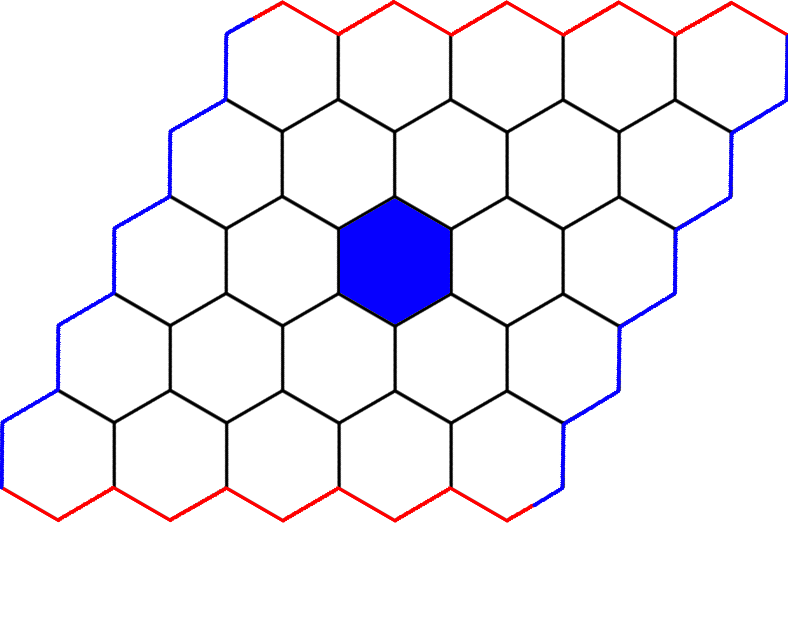
\includegraphics[width=\linewidth]{figures/example_game/ex_game_t1.png}
    \end{minipage}
    \begin{minipage}[t]{.24\linewidth}
    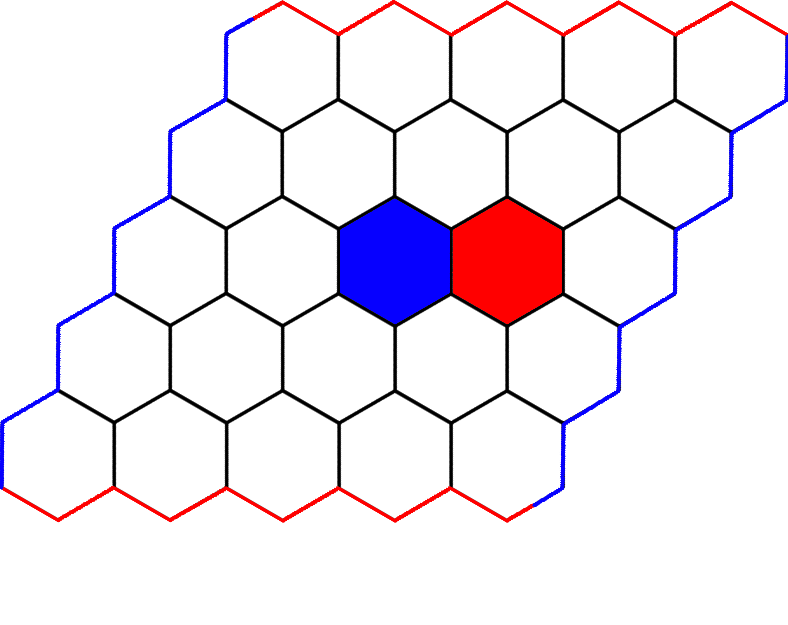
\includegraphics[width=\linewidth]{figures/example_game/ex_game_t2.png}
    \end{minipage}
    \begin{minipage}[t]{.24\linewidth}
    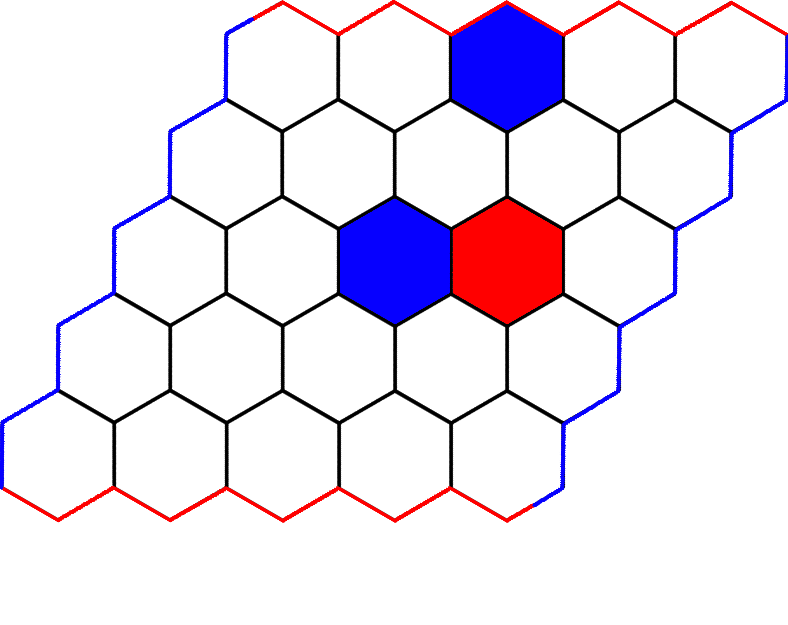
\includegraphics[width=\linewidth]{figures/example_game/ex_game_t3.png}
    \end{minipage}
    \begin{minipage}[t]{.24\linewidth}
    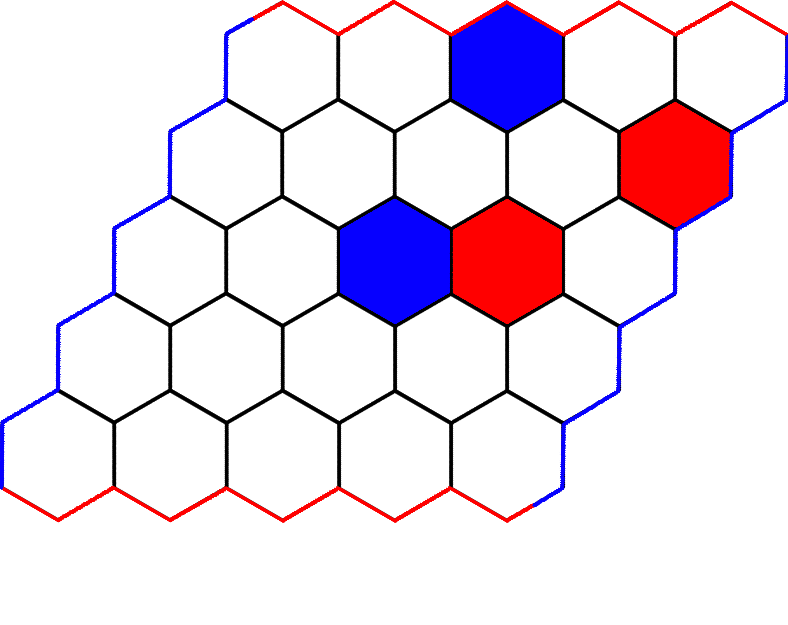
\includegraphics[width=\linewidth]{figures/example_game/ex_game_t4.png}
    \end{minipage}
    \begin{minipage}[t]{.24\linewidth}
    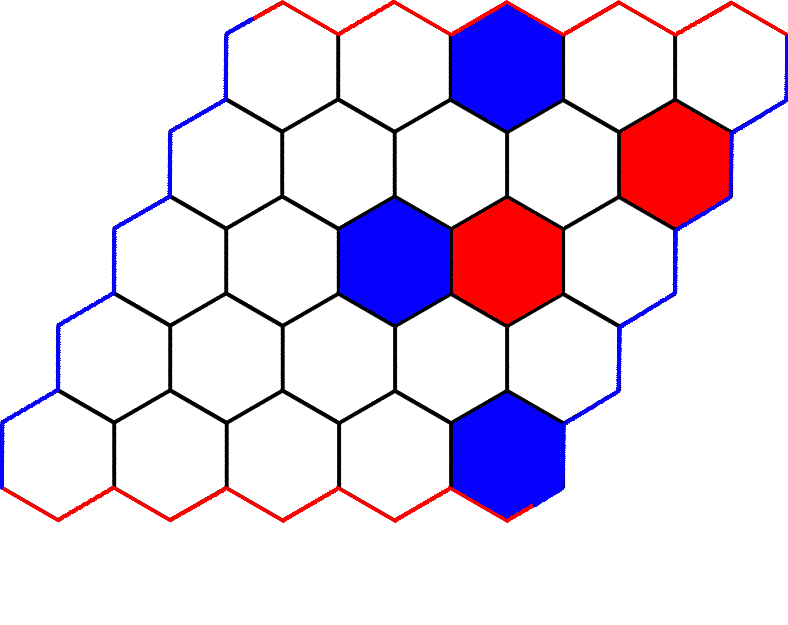
\includegraphics[width=\linewidth]{figures/example_game/ex_game_t5.png}
    \end{minipage}
    \begin{minipage}[t]{.24\linewidth}
    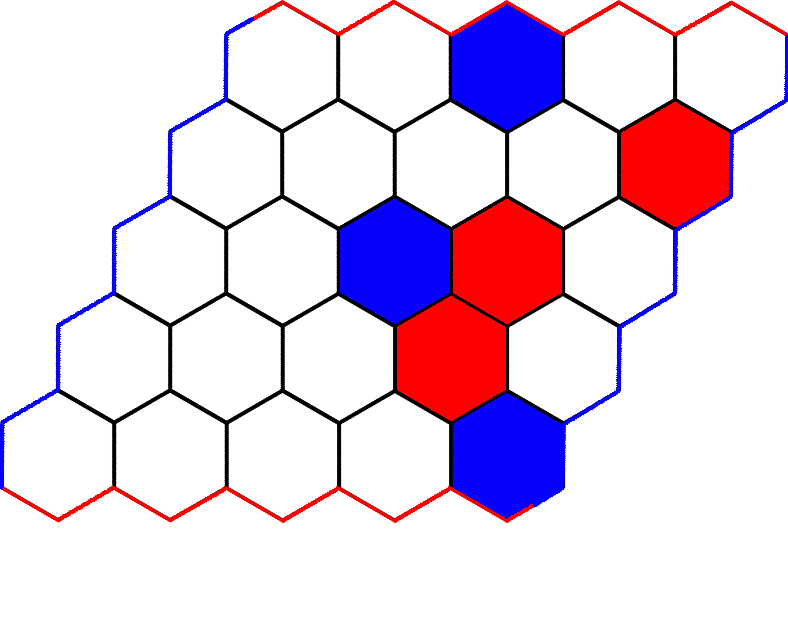
\includegraphics[width=\linewidth]{figures/example_game/ex_game_t6.png}
    \end{minipage}
    \begin{minipage}[t]{.24\linewidth}
    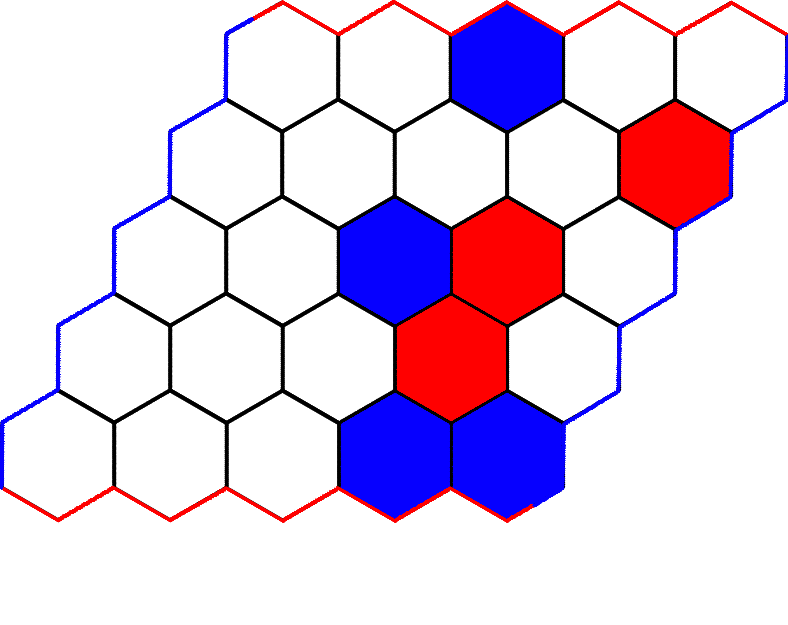
\includegraphics[width=\linewidth]{figures/example_game/ex_game_t7.png}
    \end{minipage}
    \begin{minipage}[t]{.24\linewidth}
    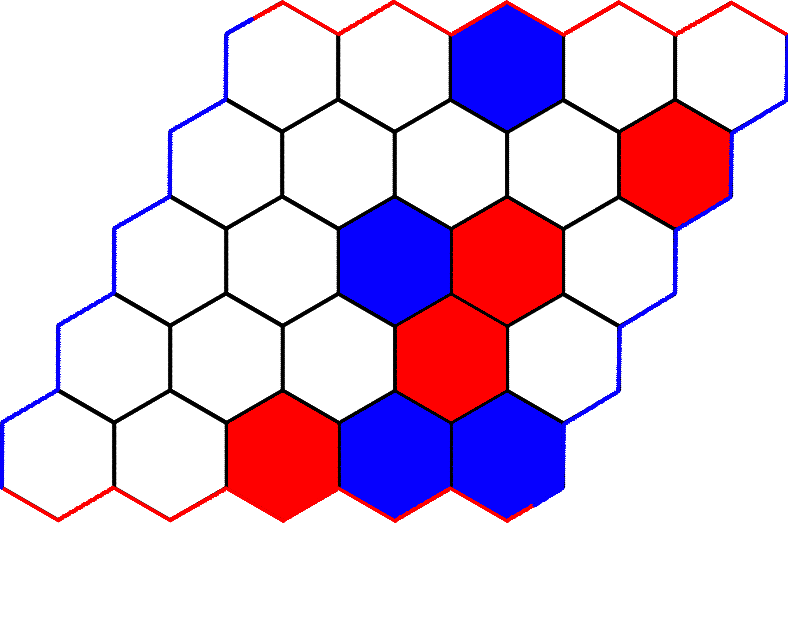
\includegraphics[width=\linewidth]{figures/example_game/ex_game_t8.png}
    \end{minipage}
    \begin{minipage}[t]{.24\linewidth}
    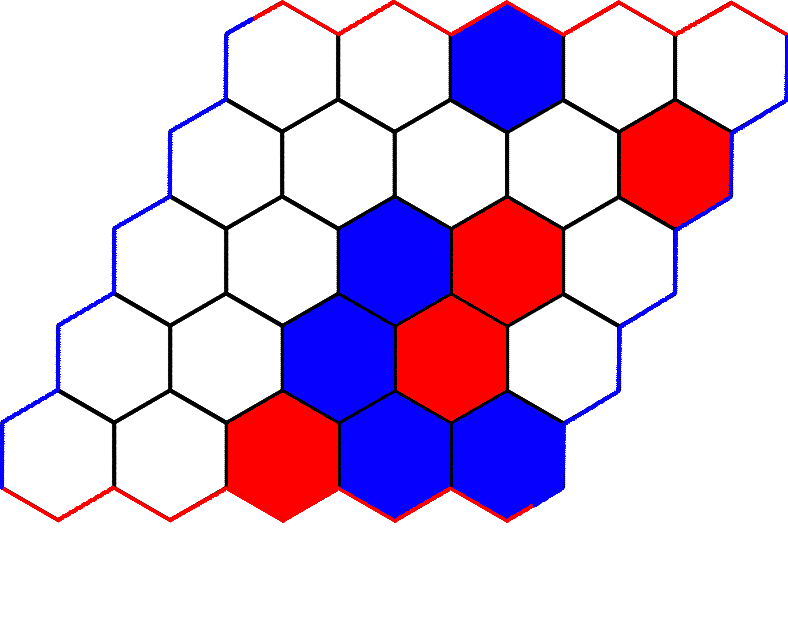
\includegraphics[width=\linewidth]{figures/example_game/ex_game_t9.png}
    \end{minipage}
    \begin{minipage}[t]{.24\linewidth}
    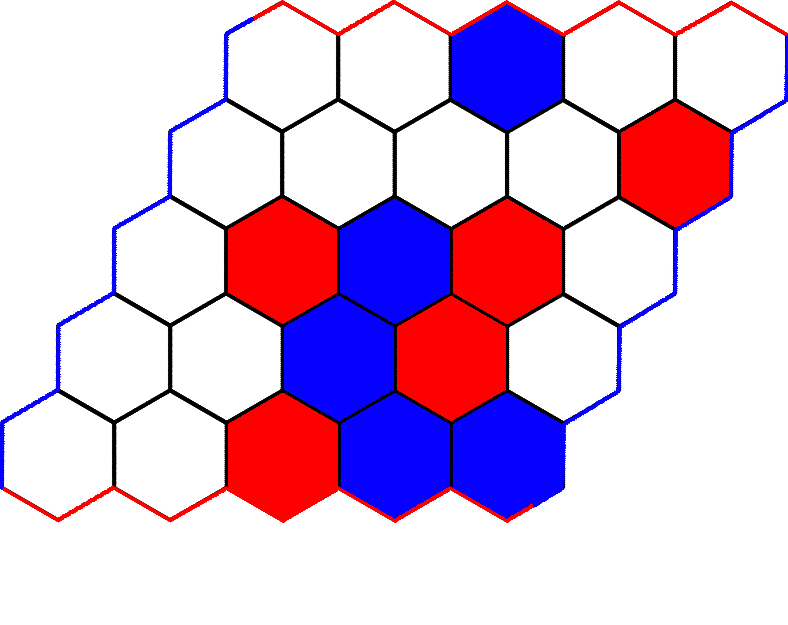
\includegraphics[width=\linewidth]{figures/example_game/ex_game_t10.png}
    \end{minipage}
    \begin{minipage}[t]{.24\linewidth}
    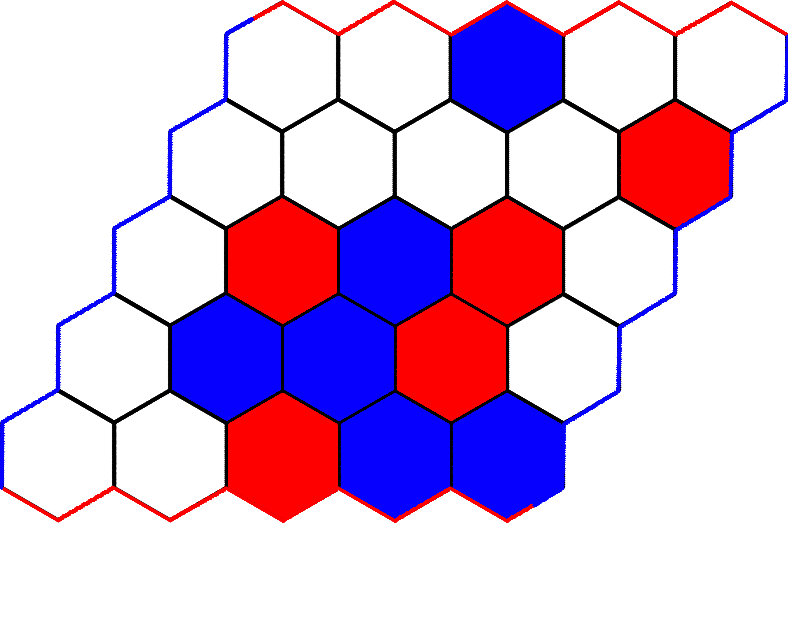
\includegraphics[width=\linewidth]{figures/example_game/ex_game_t11.png}
    \end{minipage}
    \begin{minipage}[t]{.24\linewidth}
    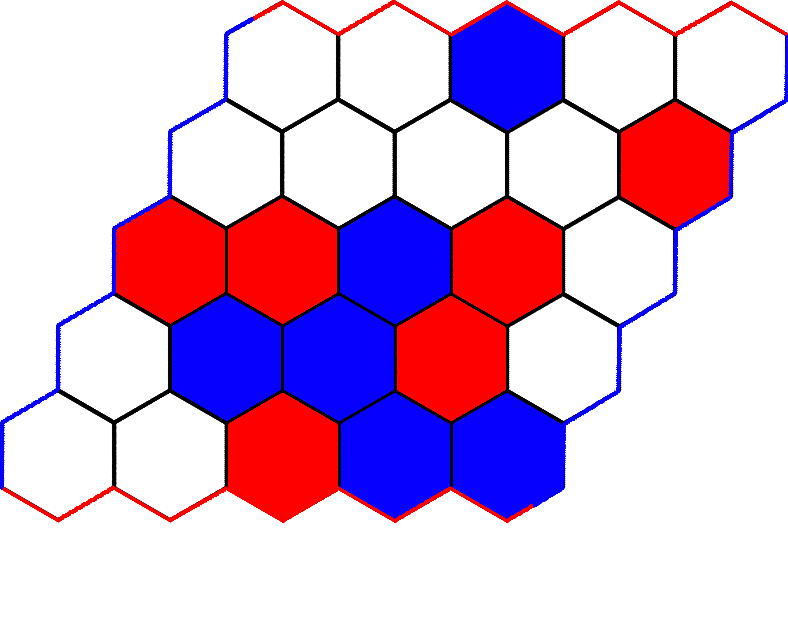
\includegraphics[width=\linewidth]{figures/example_game/ex_game_t12.png}
    \end{minipage}
    \begin{center}
    \begin{minipage}[t]{.35\linewidth}
    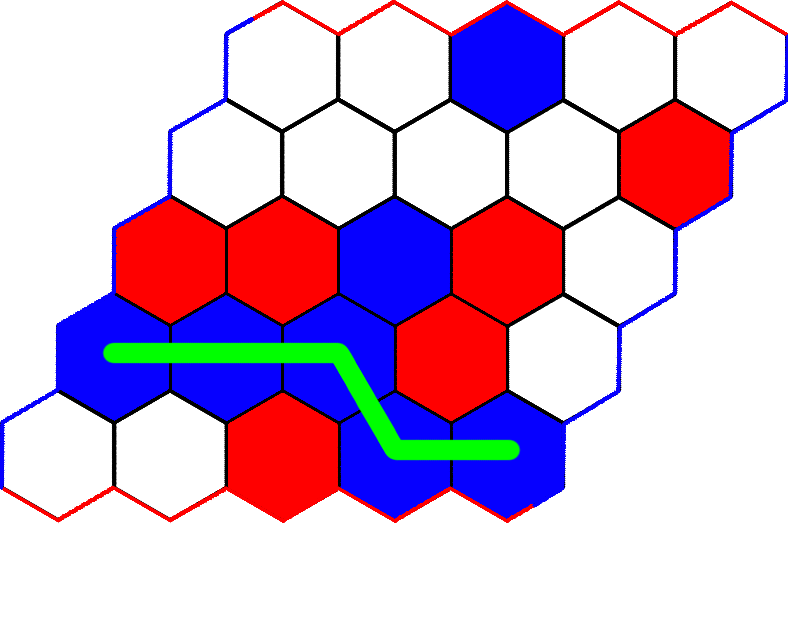
\includegraphics[width=\linewidth]{figures/example_game/ex_game_tf.png}
    \end{minipage}
    \subcaption{Example game on $5\times5$-board, where player 1 wins after 13 turns.}
    \end{center}
    \label{fig:example_game}
\end{figure}

\subsection{Why is Hex interesting?}
Hex is special type of board-game that belongs to the category called \emph{connection game}, where a player is to connect it's pieces together in some way. In hex the connection has to be made between the two sides belonging to the player. \\
The ancient Asian \textbf{GO} is also a type of connection game in which the players have to connect the pieces to capture areas of the game board. \\
One of the most interesting facts about Hex, is that a game cannot end in a draw. This has been proved using the \emph{Brouwer Fixed-Point Theorem} \cite{hexproofs1}. \\
Another interesting fact is that the mathematician John Nash has proved that for games played on symmetrical boards, there exists a winning strategy for the player starting the game. However, this does not tell us what the actual winning strategy is. \\
Using game-tree search-techniques, complete winning strategies has been found for board-sizes up to $7\times7$\footnote{https://webdocs.cs.ualberta.ca/~hayward/hex7trees/}, but for larger game-boards a general winning strategy has yet to be found.\\
This to us, makes Hex an interesting game to experiment with. \\
Even though we probably aren't going to find an optimal solution, even for small board-sizes, we might find, that it uses some interesting strategy in order to win the games. \\
Because the optimal solutions for game-boards up to size $7\times7$ has been found, it could be interesting to see if it's possible to train an \emph{ANN}, by the principles of reinforcement learning and with learning algorithms such as \emph{TD($\lambda$)} and  \emph{CMA-ES}. \\
By having the optimal solution for small board-sizes(up to $7\times7$), we are able to rate the solution against the optimal solution to see if actually learns the optimal solution. 

\section{Hex simulator}
This section describes our implementation of a simulator of the Hex game in \cpp{}. This simulator is what we use for our experiments to create a Hex AI using reinforcement learning. The reason for implementing the simulator in \cpp{} is that it is seamlessly integrated with the Shark library that we use for the machine learning parts.\footnote{\url{http://image.diku.dk/shark/}}

\subsection{Data representations and memory management}
\cpp{} requires manual memory management, and since we want to train a neural network using 10.000+ training runs we need to be careful to avoid memory leaks as this would gradually slow down the simulator. There are 2 main memory usages in the simulator, the gameboard and linesegments. The gameboard consists of \texttt{Tile} objects, and the board and tiles are allocated on the program stack at the start of the program, and reused by resetting each tile after a game. Stack allocated memory is safe in the sense that it can not lead to memory leaks, since it will be live from the moment it is allocated until the program ends.\\
A \texttt{Tile} object can be part of a \texttt{Linesegment} which is a class representing a group of connected tiles of the same color. The \texttt{Tile} class has a direct or indirect reference to the linesegment it is a part of, but the linesegments does not store the tiles that is a part of itself which spares some memory and time. The purpose of the linesegments is explained in the section about checking for winning condition. A game of Hex can be played from start to end with only 2 linesegments being used, if both players always place tiles next to their previously placed tiles, as shown in figure \ref{fig:twosegments}. But in another game where the players place tiles that are not next to any of their previous placed tiles until it is impossible to find another of such positions, there might be many linesegments. For example on a standard 11x11 rhombus shaped board there might be up to $33*2=66$ linesegments, before it is impossible to find a position that does not have any neighbours of the same color. This situation is shown in figure \ref{fig:manysegments} where any next move will be next to a neighbour of the same color, regardless of whose turn it is. After this point the amount of linesegments starts to shrink, since they will be merged with each other.\\
We decided to dynamically allocate memory for linesegments using the smart pointer \sharedptr{}\footnote{\url{https://en.cppreference.com/w/cpp/memory/shared_ptr}}. A \sharedptr{} is responsible for freeing the memory it uses, and this is done by keeping a count of references to the pointer. As soon as the last object that has a reference to the \sharedptr{} is either destroyed, or the reference is removed (perhaps by setting it to another \sharedptr{}) the memory is freed. This simplifies our code since we don't have to manually free pointers when merging linesegments or when the program ends, and it also ensures the correctness of our memory management so we have no memory leaks.

\begin{figure}
\begin{minipage}[t]{.45\linewidth}
    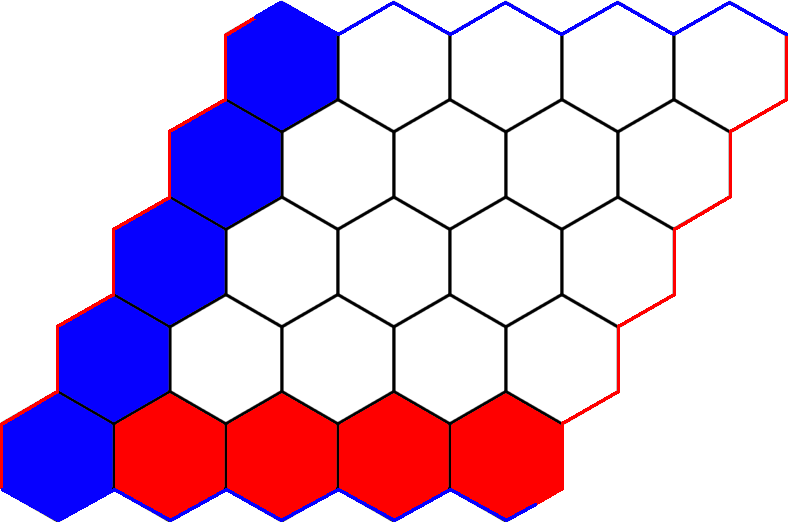
\includegraphics[width=\linewidth]{figures/hexexample_twosegments_gimp.png}
    \subcaption{Game state with 2 \texttt{Linesegments} where the player who started also won.}
    \label{fig:twosegments}
\end{minipage}
~
\begin{minipage}[t]{.45\linewidth}
    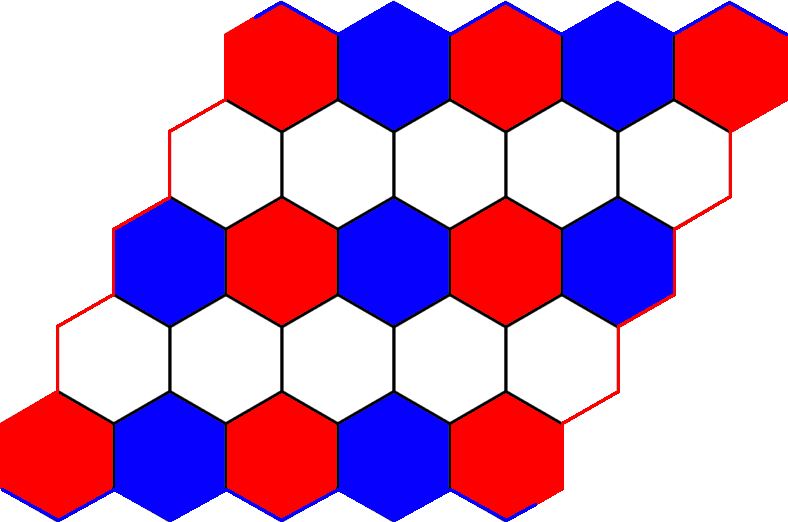
\includegraphics[width=\linewidth]{figures/hexexample_manysegments_gimp.png}
    \subcaption{Game state with 15 \texttt{Linesegments} which is the worst case for a 5x5 board. This game is not finished, but the amount of \texttt{Linesegments} will drop after this state.}
    \label{fig:manysegments}
\end{minipage}
\caption{This figure shows how the amount of \texttt{Linesegments} used depends on how the game is played. (Illustrated with GIMP) }
\end{figure}

\subsection{Game interface and basic mechanics}
The game interface is at the time of writing this subject to change, since we want to have an interface that is uniform with two other bachelor projects that have the same core focus as our project. As of now, a game can be instantiated like so (assuming the \texttt{Hex.hpp} library is properly included), \nonum \noframe
\begin{lstlisting}[language=C++]
Hex::Game game(false);
\end{lstlisting}
\setnum \setframe
The constructor argument is just a quick hack we made for debugging purposes, where true means only one player can place tiles and false means a normal game.
After instantiating a game the method takeTurn() can be called in order to advance the game.
The \texttt{takeTurn()} method is called with two 'strategies', one for each player. Depending on which player's turn it is, the corresponding strategy is used to place a new tile. The state of the game can generated, and then printed to the terminal with the method \texttt{asciiState()}.

\subsection{Strategy}



\subsection{Drawing gamestate}
% TODO: 
%% Maybe add figures that shows how it looks in the terminal
%% Talk about python program playhex.py
The \texttt{Game}-class has a method called \texttt{asciiState()} that returns a string containing the current game-state, which can be printed to the terminal. \\
We use two hexagon-shaped characters, \texttt{"\textbackslash u2b22"} and \texttt{"\textbackslash u2b21"},  from the Unicode-alphabet. 
The character \texttt{"\textbackslash u2b22"} is the solid hexagon and it represents an occupied tile. The character \texttt{"\textbackslash u2b21"} is the hollow hexagon, and represents an unoccupied tile. \\
To tell the difference between the two players hexagons, we use ANSI escape codes to color the characters red and blue. So we describe the color-coded hexagon characters as: 
\begin{figure}[H]
\begin{lstlisting}[language=C++]
const std::string m_red_color = "\033[1;31m";
const std::string m_blue_color = "\033[1;34m";
const std::string m_reset_color = "\033[0;0m";
const std::string m_hexes[3] = {
    m_blue_color + "\u2b22" + m_reset_color, // Blue
    m_red_color + "\u2b22" + m_reset_color,  // Red
    "\u2b21"                                 // Empty
};
\end{lstlisting}
\end{figure}

\subsection{Checking for win condition}
% TODO: Revise section
% We should have a better structure 
% - maybe start by showing the members of tile, and explaining that it will either have a linesegment reference or a tile reference. (never both)
A game of Hex is won if one of the players have a connected path between both of her assigned sides of the board. We don't care about finding the shortest path, any connected path will do.\\
A naive and expensive approach to checking for a winning condition would be to start at the newly placed tile, and then going through each neighbour or until the other side of the board is reached. This approach would not only be pretty expensive, and depend on the board size etc., but it would require a quite complex algorithm, which could be difficult to design and implement.\\
Instead we employ the before mentioned \texttt{Linesegment} class, and group each tile by being members of a \texttt{Linesegment}. When placing a tile we just have to update the linesegment to tell whether the game was won by placing that tile.\\ 
The \texttt{Linesegment} class is very simple, and just stores two booleans, \texttt{Connected\_A} and \texttt{Connected\_B}, and two functions, one for merging with another linesegment, and one for merging with a newly added tile. Merging just refers to OR'ing the booleans of the linesegments (or newly added tile).
\begin{lstlisting}[language=C++]
bool Merge(bool other_A, bool other_B) {
    Connected_A |= other_A;
    Connected_B |= other_B;
    return Connected_A && Connected_B;
}
\end{lstlisting}
The \texttt{Tile} class has two properties that are used to define which line segment it is a part of,
\begin{itemize}
    \item \texttt{m\_linesegment}: This is a shared pointer to a \texttt{Linesegment} object or nullptr.
    \item \texttt{m\_tile\_ref}: This is a pointer to another tile that is part of the same line segment or nullptr.
\end{itemize}
The properties are mutually exclusive, so if one is defined the other is a null pointer.
When we want to find out which line segment a tile belongs to we use the following method,
\begin{lstlisting}[language=C++]
std::shared_ptr<LineSegment> GetLineSegment() {
    if (m_linesegment != nullptr) {
        return m_linesegment;
    } else if (m_tile_ref != nullptr) {
        return m_tile_ref->GetLineSegment();
    }
}
\end{lstlisting}
An analogy for how this works is that we ask the tile, "What is your line segment?". If the tile has the reference it will give it to us, if not it will respond with, "Ask this other tile that is also part of my segment". We then ask the same question to the referenced tile until we get the line segment reference.\\ 
The critical part now is to make sure that that each tile has either a valid line- or tile reference, and that there is no cycles in the references.\\
When a new tile is placed, we check if it has any neighbours. If there are no neighbours a new line segment is created for that tile. If the tile was placed on one of the players own board edges, one of the booleans of the new line segment is set to true. If the new tile has one or more same colored neighbours we add the new tile to the line segment of the first found neighbour by setting the tile reference to point at that neighbour. If the new tile is on an edge, the corresponding line segment boolean (A or B) is set to true. For each other neighbour of the new tile that does not already share the line segment, we merge their line segments. This is done by calling a recursive function \texttt{ReferLineSegment()} which is another member of \texttt {Tile}. 
\begin{lstlisting}[language=C++]
void ReferLineSegment(Tile* newref) {
    if (m_linesegment != nullptr) {
        m_linesegment = nullptr;
        m_tile_ref = newref;
    } else if (m_tile_ref != nullptr) {
        m_tile_ref->ReferLineSegment(newref);
    }
}
\end{lstlisting}
This function will call itself recursively on the tiles tile reference, until it finds a tile that has a reference to a line segment. This reference is then removed, and instead the tile reference is set to point at the passed parameter, \texttt{newref}. So it is the last found new line segment that exists after a tile is placed, and the other line segments are all merged into it.  Figure \ref{fig:lsmerge} shows an example of two linesegments being merged. In that example there are two line segments at the beginning of a turn, and a tile is placed that touches both segments, so they are merged into one. As can be seen in the example, the line segment L2 is found first, so L2 is merged into L1 and then freed, and we end up only having L1.\\
After looping through each of the 6 neighbours, and merging any linesegments, we know instantly if the game was won or not. If the final merged linesegment has both booleans set to true, the segment has a path from one side to the other and the game is won.

\begin{figure}[t]
\begin{minipage}[t]{.45\linewidth}
    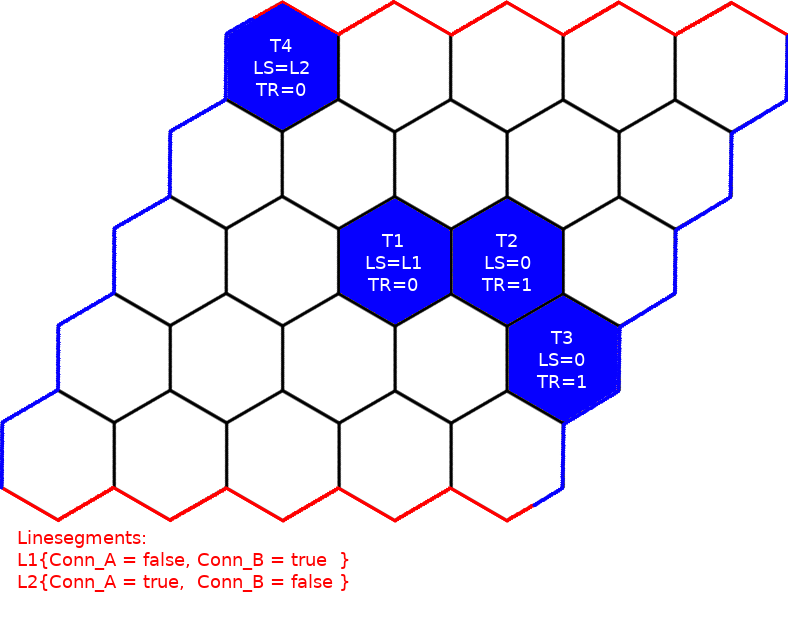
\includegraphics[width=\linewidth]{figures/hexexample_LSmerge_1.png}
    \subcaption{Before the tile T5 is placed, there are two linesegments, L1 and L2. L1 is a segment of 3 tiles, and L2 is a segment of 1 tile.}
    \label{fig:lsmerge1}
\end{minipage}
~
\begin{minipage}[t]{.45\linewidth}
    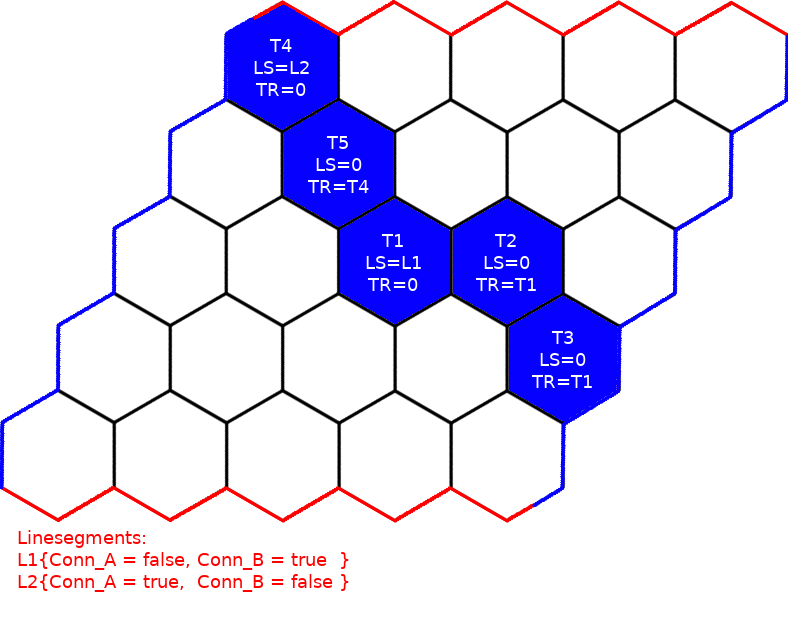
\includegraphics[width=\linewidth]{figures/hexexample_LSmerge_2.png}
    \subcaption{After placing T5, the first neighbour it finds is T4 (because it searches from top-left). T5s tile reference is thus set to T4, and T5s linesegment reference is null.}
    \label{fig:lsmerge2}
\end{minipage}
\\\\
\begin{center}
\begin{minipage}[t]{\linewidth}
    \begin{center}
    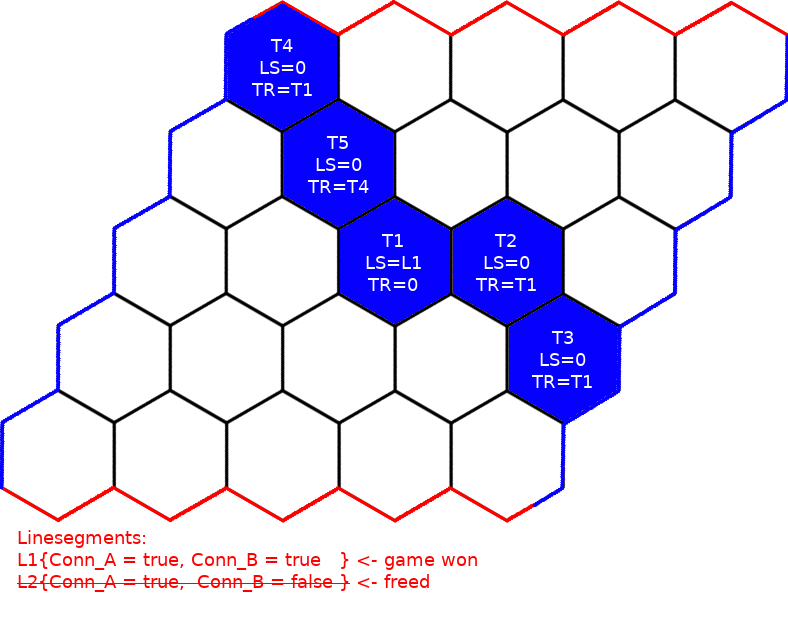
\includegraphics[width=.45\linewidth]{figures/hexexample_LSmerge_3.png}
    \end{center}
    \subcaption{The next (and last) neighbour it finds is T1, so \texttt{ReferenceLineSegment(T1)} is called on T5, and since T5 have a tile reference, the function is called again on T4. This tile has a linesegment reference, so that is set to null, and its tile reference is set to T1 (from the \texttt{ReferenceLineSegment} argument). Now there's only one linesegment, and this linesegment is connected to both of blues sides, so blue wins the game. Also shown is the fact that every reference to L2 is lost, so the smart pointer is freed.}
    \label{fig:lsmerge3}
\end{minipage}
\end{center}
\caption{Example of two linesegments being merged after a tile (T5) is placed that connects them. (Illustrated with GIMP)}
\label{fig:lsmerge}
\end{figure}



\begin{thebibliography}{9}
\bibitem{hexproofs1} 
Gale, David. 
\textit{“The Game of Hex and the Brouwer Fixed-Point Theorem.”}. 
The American Mathematical Monthly, vol. 86, no. 10, 1979, pp. 818–827. JSTOR, www.jstor.org/stable/2320146.

 

\end{thebibliography}



\end{document}